% !TEX root = _individual/implementation.tex

%%%%%%%%%%%%%%%%%%%%%%%%%%%%%%%%%%%%%%%%%%%%%%%%%%%%%%%%%%%%%%%%%%%%%%%%%%%%%%%%
\chapter{Low-order discretization schemes} \label{chap:implementation}

The use of anisotropic diffusion tensors is not new, nor is the search for
accurate discretizations. In this dissertation, we only consider a structured
two-dimensional Cartesian mesh, where all cells are quadrilaterals, and each
cell connects (in
the interior) to four adjacent cells through four faces, and each face is
perpendicular to one of the coordinate system axes.

Because of this simplified problem space, we need not implement the more
complex Support Operators Methods \cite{Mor1998,Run2006}. But the complexity is
not just a burden on the programmer; those methods increase the number of
unknowns and the change the structure of the resulting system of equations,
meaning longer solution times for the user. With this in mind, we seek in this
chapter to find simple but accurate methods of solving the low-order system of
equations for Anisotropic Diffusion on Cartesian meshes.

%%%%%%%%%%%%%%%%%%%%%%%%%%%%%%%%%%%%%%%%%%%%%%%%%%%%%%%%%%%%%%%%%%%%%%%%%%%%%%%%
\section{Introduction}

Because the semi-implicit gray TRT formulation can be expressed as a
steady-state transport equation (see \S\ref{sec:trtLinearizedComments}), for
simplicity we will present these discretizations without time dependence.

The steady-state particle conservation equation is
\begin{equation}\label{eq:ssConservation}
  \grad \vd \vec{F}(\vec{x}) + \sigma_a(\vec{x}) \phi(\vec{x}) =
  q(\vec{x})\,,\qquad \vec{x} \in V\,.
\end{equation}
The first step in a simple differencing scheme is to assume that the unknown
(in this case, $\phi$) is constant over a single cell, represented in
Fig.~\ref{fig:cellDiagram}. We also assume that the opacity and source are
constant over the cell, which, for TRT, means assuming the material temperature
is constant over a cell. Integrating Eq.~\eqref{eq:ssConservation} over cell
$i,j$ and using the divergence theorem gives
\begin{equation} \label{eq:ssConservationDisc}
  %\sum_{f\in \{L,R,B,T\}} \int_f \vec{n}_f \vd \vec{F} \ud A
  \Delta_{x,i} \left( F_T^y - F_B^y \right)
+ \Delta_{y,j} \left( F_R^x - F_L^x \right)
+ \Delta_{x,i}\Delta_{y,j} \sigma_{a,i,j} \phi_{i,j}
= \Delta_{x,i}\Delta_{y,j} q_{i,j}\,.
\end{equation}
Here, $F_A^b$ is the leakage (radiation flux) from cell $i,j$ through face $A$
along the $b$ axis. The methods presented in the following sections provide
different closures for the leakages in terms of the other unknowns. They all
serve to approximate the ``Fick's law'' of anisotropic diffusion,
\begin{equation*}
  \vec{F} = - \Dtens \vd \grad \phi
  = -
  \begin{bmatrix}
    D^{xx} & D^{yx} \\
    D^{xy} & D^{yy}
  \end{bmatrix}
  \begin{bmatrix}
    \tpder{\phi}{x} \\
    \tpder{\phi}{y}
  \end{bmatrix}
  = 
  \begin{bmatrix}
    - D^{xx} \tpder{\phi}{x}
    - D^{yx} \tpder{\phi}{y} \\
    - D^{yy} \tpder{\phi}{y}
    - D^{xy} \tpder{\phi}{x}
  \end{bmatrix}
  \,.
\end{equation*}
Because the diffusion matrix is symmetric, $D^{yx}=D^{xy}$.

\begin{figure}[htb]
  \centering
  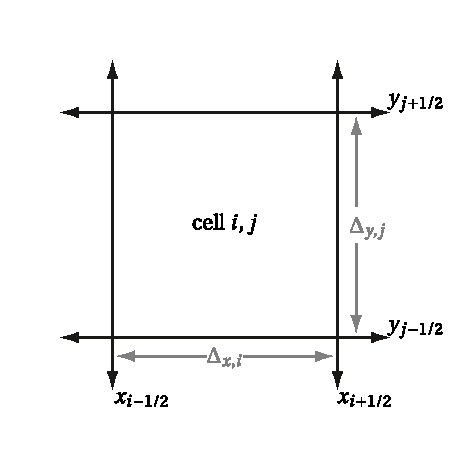
\includegraphics{cell-diagram}
  \caption{Diagram of cell $i,j$.}
  \label{fig:cellDiagram}
\end{figure}

To preserve particles, it's necessary that $F_T^y$ from cell $i,j$ is equal to
$F_B^y$ from cell $i,{j+1}$, and the same from the other directions.

%%%%%%%%%%%%%%%%%%%%%%%%%%%%%%%%%%%%%%%%%%%%%%%%%%%%%%%%%%%%%%%%%%%%%%%%%%%%%%%%
\section{Neglecting transverse diffusion}

Perhaps the simplest way to discretize the anisotropic diffusion equation is by
neglecting the off-diagonal terms of the diffusion tensor that imply transverse
leakage.

In certain simple problems, this is not an approximation. As long as the
opacity is invariant with respect to one of the coordinate system's axes, the
transport solution for $f$ will only change along one axis, and the
off-diagonal terms are zero. Larsen and Trahan's VHTR test problem
\cite{Lar2009c} is an example of such a geometry.

%%%%%%%%%%%%%%%%%%%%%%%%%%%%%%%%%%%%%%%%%%%%%%%%%%%%%%%%%%%%%%%%%%%%%%%%%%%%%%%%
\section{Gol'din-style discretization}

\cite{Val2002}

\begin{figure}[htb]
  \centering
  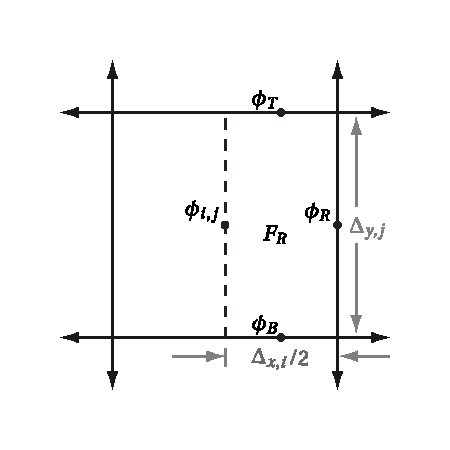
\includegraphics{goldin-righthalf}
  \caption{Right half of cell $i,j$.}
  \label{fig:goldinRight}
\end{figure}

%%%%%%%%%%%%%%%%%%%%%%%%%%%%%%%%%%%%%%%%%%%%%%%%%%%%%%%%%%%%%%%%%%%%%%%%%%%%%%%%
\section{Nine-point stencil}

Fig.~\ref{fig:cellAnisoLeakage} shows the leakage out of cell $i,j$ through the
right face.
\begin{figure}[htb]
  \centering
  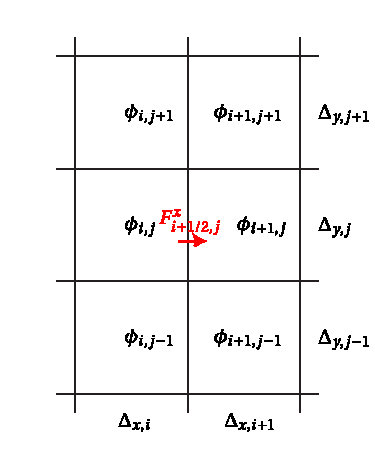
\includegraphics{cell-leakage-right}
  \caption{Diagram showing the radiation exiting interior cell $i,j$ through the
  right face.}
  \label{fig:cellAnisoLeakage}
\end{figure}
We evaluate the face-averaged normal component of the flux,
$F_{i+1/2,j}^x \equiv \int_{y_{j-1/2}}^{y_{j+1/2}} \vec{F} \vd \vec{n} \ud
y$, from both cell $i,j$ and cell $i+1,j$, and set them equal to each other.
Solving for $F_{i+1/2,j}^x$ gives
\begin{equation} \label{eq:cellAnisoFlux}
  F_{i+1/2,j}^{x} \approx
  - \frac{D^{xx}_{i+1/2,j}}{\Delta_{x,i+1/2}}
  \left[ 
    \left( \phi_{i+1,j} - \phi_{i,j} \right)
  + \frac{D^{xy}_{i,j}/D^{xx}_{i,j}}{2/\Delta_{x,i}}
    \pder{\phi}{y} \Bigg|_{x_{i+1/2}^-}
  + \frac{D^{xy}_{i+1,j}/D^{xx}_{i+1,j}}{2/\Delta_{x,i+1}}
    \pder{\phi}{y} \Bigg|_{x_{i+1/2}^+}
  \right]
\end{equation}
where $\tpder{\phi}{y} |_{x_{i+1/2}^-}$ is the transverse derivative of
$\phi$ on the left side of the face, and $\tpder{\phi}{y} |_{x_{i+1/2}^+}$ is
the transverse derivative as viewed from the right side of the face.
The harmonic-averaged diffusion coefficient is
\begin{equation} \label{eq:cellEdgeDHarmonic}
  \frac{D^{xx}_{i+1/2,j}}{\Delta_{x,i+1/2}} \equiv \left[
  \frac12 \left( \frac{D^{xx}_{i,j}}{\Delta_{x,i}} \right)\inv
 + \frac12 \left( \frac{D^{xx}_{i+1,j}}{\Delta_{x,i+1}} \right)\inv
  \right]\inv\,.
\end{equation}

If $D^{xy}$ were zero for both cells, and $D^{xx}=D^{yy}$,
Eq.~\eqref{eq:cellAnisoFlux} would reduce to
the standard cell-centered finite difference discretization so well known to
nuclear engineering students.

Now, in our first nine-point stencil, we approximated
\begin{equation*}
  \pder{\phi}{y} \Bigg|_{x_{i+1/2}^-} \approx \frac{\phi_{i,j+1} -
  \phi_{i,j-1}}{\tfrac12 \Delta_{y,j+1} + \Delta_{y,j} + \tfrac12
  \Delta_{y,j-1}}
\end{equation*}
in the interior of the problem and discarded the term near the boundaries. (The 
$\tpder{\phi}{y} |_{x_{i+1/2}^+}$ term is the same but replacing $i\to i+1$.)
An improvement is to approximate the case on the top boundary with
\begin{equation*}
  \pder{\phi}{y} \Bigg|_{x_{i+1/2}^-} \approx \frac{\phi_{i,j} -
  \phi_{i,j-1}}{\tfrac12 \Delta_{y,j} + \tfrac12 \Delta_{y,j-1} }
\end{equation*}
and the case on the bottom boundary with 
\begin{equation*}
  \pder{\phi}{y} \Bigg|_{x_{i+1/2}^-} \approx \frac{\phi_{i,j+1} -
  \phi_{i,j}}{\tfrac12 \Delta_{y,j+1} + \tfrac12 \Delta_{y,j} }
\end{equation*}

We can also approximate this derivative with approximate cell-edge values. In
the finite difference method, an intermediate cell-edge $\phi$ helps represent
the slope normal to the edge. It is eliminated in the process of finding
$\vec{F}\vd\vec{n}$, but if there is no transverse term, it is possible to
solve for the cell-edge $\phi$ in terms of the two cell-centered $\phi$. Let us
consider the finite difference approximation coupling two cells:
\begin{equation*}
  F = - D_0 \frac{\phi_{1/2} - \phi_0}{\Delta_0/2}
  \qquad\text{and}\qquad
  F = - D_1 \frac{\phi_{1} - \phi_{1/2}}{\Delta_1/2}\,.
\end{equation*}
Multiplying the left equation by $\Delta_0 / D_0$ and the right equation by
$\Delta_1 / D_1$,
\begin{equation*}
  -\frac{\Delta_0/2}{D_0 } F = \phi_{1/2} - \phi_0
  \qquad\text{and}\qquad
  -\frac{\Delta_1/2}{D_1 } F = \phi_{1} - \phi_{1/2}
\end{equation*}
adding them eliminates gives the standard finite-difference approximation for $F$,
\begin{equation*}
  F = - \left( \frac{\Delta_0/2}{D_0 } + \frac{\Delta_1/2}{D_1 } \right)\inv
  \left( \phi_1 - \phi_0 \right),
\end{equation*}
and subtracting the second from the first gives
\begin{equation*}
 -\frac{\Delta_0/2}{D_0 }F + \frac{\Delta_1/2}{D_1 } F
 = 2 \phi_{1/2}-(\phi_0+\phi_1)\,.
\end{equation*}
Defining $ d_i \equiv \frac{\Delta_i}{D_i}$ for $i=0,1$ for brevity, then
\begin{equation*}
  \frac12 F (d_1 - d_0)
 = 2 \phi_{1/2}-(\phi_0+\phi_1)
  \qquad\text{and}\qquad
 F = -2\left( d_1 + d_0 \right)\inv (\phi_1 - \phi_0)\,.
\end{equation*}
Substituting $F$ into the left equation,
\begin{align*}
  \left( d_1 + d_0 \right)\inv\left(d_1 - d_0\right) (\phi_1 - \phi_0)
  &= 2 \phi_{1/2}-(\phi_0+\phi_1)
  \\
 \frac12 \left[ 1 - \frac{d_1 - d_0}{d_1 + d_0} \right] \phi_1
+ \frac12 \left[ 1 + \frac{d_1 - d_0}{d_1 + d_0} \right] \phi_0
 &= \phi_{1/2}
  \\
 \frac{d_0}{d_1 + d_0} \phi_1
+ \frac{d_1}{d_1 + d_0} \phi_0
 &= \phi_{1/2}\,.
\end{align*}

For our case in anisotropic diffusion, we want to approximate 
\begin{equation*}
  \pder{\phi}{y} \Bigg|_{x_{i+1/2}^-} \approx \frac{\phi_{i,j+1/2} -
  \phi_{i,j-1/2}}{\Delta_{y,j}} \,.
\end{equation*}
In evaluating these cell-edge $\phi$ we neglect the transverse leakage (as
leaving them in would add unknowns on more cell faces) and apply the previous
result:
\begin{equation*}
  \phi_{i,j+1/2} \approx
  \frac{D_{i,j}^{yy} / \Delta_{y,j}}{D_{i,j+1}^{yy} / \Delta_{y,j+1} +
  D_{i,j}^{yy} / \Delta_{y,j}} \phi_{i,j+1}
+ \frac{D_{i,j+1}^{yy} / \Delta_{y,j+1}}{D_{i,j+1}^{yy} / \Delta_{y,j+1} +
D_{i,j}^{yy} / \Delta_{y,j}} \phi_{i,j} \,.
\end{equation*}
Subtracting one from the $j$ indices gives the corresponding equation for the
bottom face:
\begin{equation*}
  \phi_{i,j-1/2} \approx
  \frac{D_{i,j-1}^{yy} / \Delta_{y,j-1}}{D_{i,j}^{yy} / \Delta_{y,j} +
  D_{i,j-1}^{yy} / \Delta_{y,j-1}} \phi_{i,j}
+ \frac{D_{i,j}^{yy} / \Delta_{y,j}}{D_{i,j}^{yy} / \Delta_{y,j} +
D_{i,j-1}^{yy} / \Delta_{y,j-1}} \phi_{i,j-1} \,.
\end{equation*}
If cell $i,j$ is in the interior, 
\begin{equation*}
  \pder{\phi}{y} \Bigg|_{x_{i+1/2}^-} \approx \frac{\phi_{i,j+1/2} -
  \phi_{i,j-1/2}}{\Delta_{y,j}} \,,
\end{equation*}
or if it is on the top boundary,
\begin{equation*}
  \pder{\phi}{y} \Bigg|_{x_{i+1/2}^-} \approx \frac{\phi_{i,j} -
  \phi_{i,j-1/2}}{\Delta_{y,j} / 2} \,,
\end{equation*}
or if it is on the bottom boundary,
\begin{equation*}
  \pder{\phi}{y} \Bigg|_{x_{i+1/2}^-} \approx \frac{\phi_{i,j+1/2} -
  \phi_{i,j}}{\Delta_{y,j} / 2} \,.
\end{equation*}

If the anisotropic diffusion coefficients are homogeneous and the grid is
uniform, this expression for $\tpder{\phi}{y}$ is exactly equivalent to the
simpler one.

\begin{figure}[htb]
  \centering
  %\hspace{-.6in}
  \subfigure[Diagonal-only anisotropic]{
  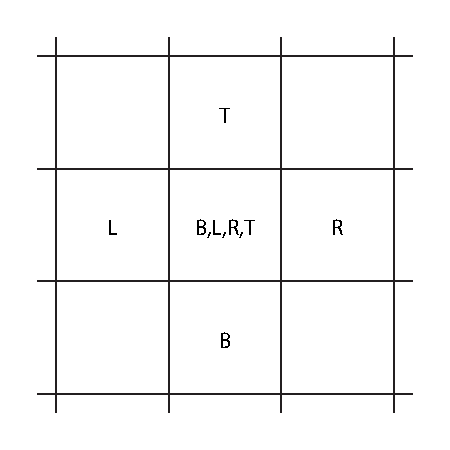
\includegraphics{diaganiso-leakage-terms}
  }
  %\hspace{-.2in}
  \subfigure[Cell anisotropic]{
  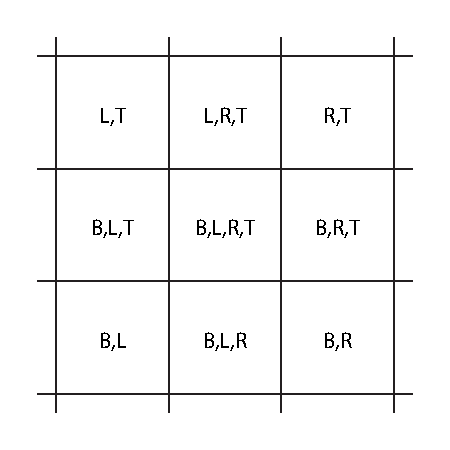
\includegraphics{cellaniso-leakage-terms}
  }
  %\hspace{-.6in}
  \caption{Stencils for $- \grad \vd \Dtens \grad \phi$ showing contribution
  from the leakage terms of each face of the center cell.}
  \label{fig:anisoStencils}
\end{figure}


